\documentclass[10pt,fleqn]{article} % Default font size and left-justified equations
\usepackage{import}
\usepackage[%
    pdftitle={Chaine d'information},
    pdfauthor={Geoffrey Vaquette}]{hyperref}
\subimport{../../../../style/}{preambule.tex}
%\fichetrue
\fichefalse
\proftrue
%\proffalse
%\tdtrue
\tdfalse
\courstrue
%\coursfalse
\subimport{../../../../style/}{new_style}
\subimport{../../../../style/}{macros_SII}
\subimport{../../../../style/}{preambule_trou.tex}

\usepackage{siunitx}
\sisetup{inter-unit-product = \ensuremath { { } \cdot { } } }
% -------------------------------------
% Déclaration des titres
% -------------------------------------

\def\discipline{Enseignement \\Technologique \\ Transversal}
\def\xxtete{Enseignement Technologique Transversal}

\def\classe{1 STI2D}
\def\xxnumpartie{Séquence 2}
\def\xxpartie{Modélisation des énergies au sein d'un système}

\def\xxnumchapitre{Séance 2}
\def\xxchapitre{\hspace{.12cm} Énergies, Puissances et rendement}

\def\xxposongletx{2}
\def\xxposonglettext{1.45}
\def\xxposonglety{23}
\def\xxonglet{Seq. 2 -- Se. 2}

\def\xxactivite{Cours}
\def\xxauteur{\textsl{Geoffrey Vaquette}}

\def\xxcompetences{%
\textsl{%
\textbf{Savoirs et compétences :}
\begin{itemize}[label=\ding{112},font=\color{ocre}]
\item CO2.1	Identifier les flux et la forme de l'énergie, caractériser ses transformations et/ou modulations et estimer l'efficacité globale d'un système.
\end{itemize}
%
}}

\def\xxfigures{
\begin{center}
%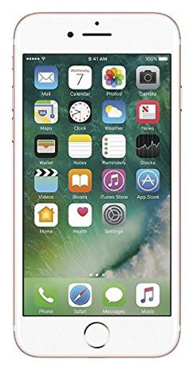
\includegraphics[height=4cm]{images/smartphone.png} \\
%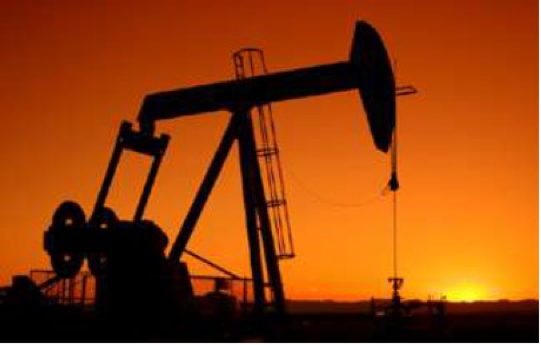
\includegraphics[height=4cm]{images/petrole.png} \\
%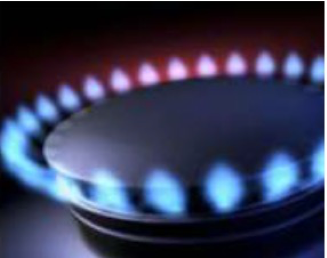
\includegraphics[height=4cm]{images/gaz.png} \\
\end{center}
}%figues de la page de garde
\def\xxpied{%
Chaine d'information) \xxactivite%
}

%---------------------------------------------------------------------------

\renewcommand{\RemplirTrou}{true}
\begin{document}
\chapterimage{png/numerique}
\subimport{../../../../style/}{new_pagegarde}

\section{Chaine d'information}

Comme on l'a vu précédemment, un système agit sur une matière d'oeuvre en vue de 
lui apporter une valeur ajoutée. Pour cela, le système a besoin de connaître des 
informations (ordres, état des capteurs) pour fonctionner. 

On peut modéliser la partie d'un syustème qui gère les informations par ce qu'on 
appellera la \textbf{chaine d'information}. 

\begin{definition}
  La chaîne d'information permet de modéliser la façon dont un système \textbf{acquiert}, \textbf{traite} et 
  \textbf{communique} les informations.  
\end{definition}

Elle est modélisable par une série de trois blocs : 
\begin{description}
  \item[Acquérir : ] Modélise les éléments qui captent de l'information 
  extérieure au système. 
  \item[Traiter : ] Modélise les éléments qui traitent (interprètent, modifient, ...) 
  les informations.
  \item[Communiquer : ] Modélise les éléments qui servent à la communication du 
  système avec l'extérieur. 
\end{description}

\subsection{Acquérir}
Pour acquérir de l'information en provenance de l'extérieur, les systèmes sont 
équipés de capteurs. Ces capteurs ont pour fonction de traduire une information  
physique dans un langage compréhensible par un système numérique (la partie commande par 
exemple).

\subsubsection{Les capteurs Tout ou Rien (TOR)}
Les capteurs Tout ou Rien (TOR) fournissent une information binaire (à deux 
valeurs). Comme leur nom l'indique, ils donnent une information sur la présence 
(tout) ou l'absence (rien) d'un 


\end{document}
